\subsection{Instruction Structure} \label{subsec:instruction-structure}

Based on the VM instruction set defined in Section \ref{subsec:instruction-set}, the VM is able to execute programs. OlaVM proof system can constrain the semantics of each instruction according to the execution trace of the VM to ensure that the program has been executed correctly. However, we also need to ensure that the actual program being executed has not been maliciously modified, meaning, we have to ensure it executed the original, correct program. As for how to check that the instructions involved in the execution trace are all present in the original program fragment and if they are executed in the correct \verb|pc| order, we've decided to compare whether or not each instruction in the execution trace is included in the original program. In order to do that, we encode each instruction, then checking if the encoding of the execution instruction is included in the encoding of the program instruction.

Instruction encoding form as shown in Figure \ref{fig:instruction-encoding} with each instruction encoding occupying 32 bits.
\begin{figure}[!ht]
    \centering
    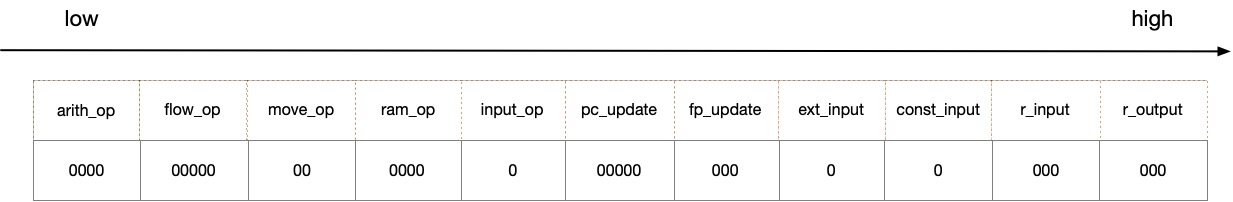
\includegraphics[width=\textwidth]{instruction-encode.jpg}
    \caption{Instruction encoding}
    \label{fig:instruction-encoding}
\end{figure}

As shown in Table \ref{fig:instruction-encoding}, the instruction will set the bit value of each used item to 1 and set the unused item to 0 when encoding. The specific meaning of each item is explained as follows:
\begin{itemize}
    \item \verb|arith_op| is the logic of arithmetic operation, which occupies 4 bits and is used to select the 4 instructions of \verb|ADD|, \verb|SUB|, \verb|MUL| and \verb|DIV|;
    \item \verb|flow_op| is the control logic, which occupies 5 bits and is used to indicate the selection of control-related instructions;
    \item \verb|mov_op| is the register move logic, which occupies 2 bits and is used to indicate the selection of \verb|mov|-related instructions;
    \item \verb|ram_op| is the operation logic of memory and storage, which occupies 4 bits and is used to indicate the selection of specific operations;
    \item \verb|input_op| is the input logic, which occupies 1 bit and is used to indicate the selection of the program to read the input from outside;
    \item \verb|pc_update|, occupying 5 bits, is used to indicate the relevant logic of \verb|pc| update. \verb|pc| can be updated through \verb|flow_op| or updated normally, and the \verb|pc_update| value of normal update is 00000;
    \item \verb|fp_update|, occupying 3 bits, is used to indicate whether \verb|fp| is updated. Instructions \verb|CALL|, \verb|RET| and \verb|END| will update \verb|fp|;
    \item \verb|ext_input|, occupying 1 bit, is used to indicate whether there is an external input;
    \item \verb|const_input|, occupying 1 bit, is used to indicate whether the instruction has immediate value input;
    \item \verb|r_input|, occupying 3 bits, is used to indicate whether the instruction read input values from three registers \verb|r0|, \verb|r1| and \verb|r2|;
    \item \verb|r_output|, occupying 3 bits, is used to indicate whether the instruction will update the value of three registers \verb|r0|, \verb|r1| and \verb|r2|.
\end{itemize}

\noindent
The encoding forms of \verb|arith_op| are
\begin{lstlisting}
0001 -> ADD
0010 -> SUB
0100 -> MUL
1000 -> DIV
\end{lstlisting}
The encoding forms of \verb|flow_op| are
\begin{lstlisting}
00001 -> JMP
00010 -> CJMP
00100 -> CALL
01000 -> RET
10000 -> END
\end{lstlisting}
The encoding forms of \verb|mov_op| are
\begin{lstlisting}
01 -> MOV
10 -> MOVI
\end{lstlisting}
The encoding forms of \verb|ram_op| are
\begin{lstlisting}
0001 -> MSTORE
0010 -> MLOAD
0100 -> SSTORE
1000 -> SLOAD
\end{lstlisting}
The encoding form of \verb|input_op| is
\begin{lstlisting}
1 -> READ
\end{lstlisting}
The encoding forms of \verb|pc_update| are
\begin{lstlisting}
00001 indicates pc changes caused by JMP
00010 indicates pc changes caused by CJMP
00100 indicates pc changes caused by CALL
01000 indicates pc changes caused by RET
10000 indicates pc changes caused by END
\end{lstlisting}
The encoding forms of \verb|pc_update| are
\begin{lstlisting}
01 indicates the change of the fp register pointer caused by the CALL instruction
10 indicates the change of the fp register pointer caused by the RET instruction
\end{lstlisting}
The encoding forms of \verb|fp_update| are
\begin{lstlisting}
001 indicates the content change of the fp register caused by the CALL instruction
010 indicates the content change of the fp register caused by the RET instruction
100 indicates the content change of the fp register caused by the END instruction
\end{lstlisting}
The encoding forms of \verb|ext_input| are
\begin{lstlisting}
1 indicates the existence of external input data
\end{lstlisting}
The encoding form of \verb|const_input| is
\begin{lstlisting}
1 indicates that mov instruction has immediate value input
\end{lstlisting}
The encoding form of \verb|r_input| is as follows
\begin{lstlisting}
001/010/100 indicates the input of register r0, r1 and r2 respectively
\end{lstlisting}
The encoding form of \verb|r_output| is as follows
\begin{lstlisting}
001/010/100 indicates the output of register r0, r1 and r2 respectively
\end{lstlisting}

The description above contains instruction encoding forms, without immediate value encoding forms of the instruction. If an instruction involves immediate value, we will encode the immediate value after the instruction. At this time, \verb|pc| is increased by the size of instruction each time, namely \verb|pc = pc + instruction_size|.

With the above code rules, we can prove that the executed program fragment is indeed derived from the original program. In order to ensure the execution of the correct program sequence in case of program jumps, an additional \verb|pc| code to the instruction is required to prove the program is executed in the correct sequence.
